\section{Performance Analysis}
\label{analysis}
% %TODO: is it better to consider a fixed length packet or variable length?
% %TODO: Whether this hypothesis should be kept? Radio link conditions are ideal and data reporting is finished in the first transmission. 
A comparative performance analysis between traditional RACH and our proposal (network integrated M2M-orientated polling service) is presented in this section. We focus on the consumption of RBs  (used for data transmission and signaling) and the minimum number of RNTI, for both methods.

\subsection{System model}
\begin{figure}[!t]
	\centering
	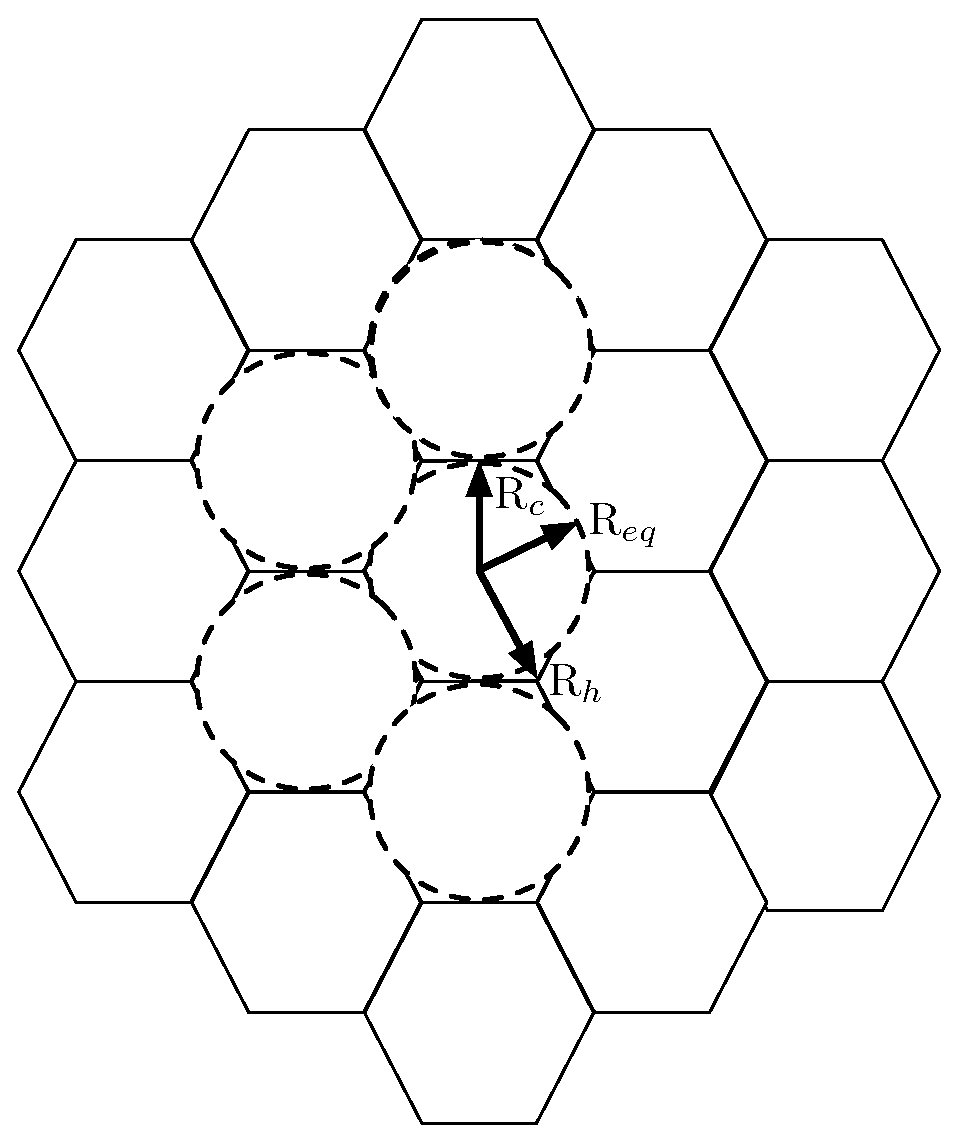
\includegraphics[scale=0.5]{Chapter6/Figures/hexagone_grid}
	\caption{The studied hexagonal grid network topology}
	\label{fig:hexagone_grid}
\end{figure}

We consider a regular hexagonal network whose topology is illustrated in Fig.~\ref{fig:hexagone_grid}, where $R_{h}$ refers to the hexagonal radius and $R_c$ denotes the half distance between two adjacent eNBs. We assume that all the eNBs have omnidirectional antenna so that each eNB covers a single cell. All eNB transmit with the same power.

The amount of MTC devices served by each eNB, denoted by $N_d$, is assumed to be very large. These devices are static and periodically sending data to remote servers. The device reporting period $T$ is assumed to be a random variable whose distribution can be of any type. To reduce the reporting collision rate, the report moment for each device is chosen uniformly between time interval $\left[ 0, T\right] $. 

Fractional power control is taken into account in this model. The path-loss is partially compensated by the power control scheme. The power compensation factor is denoted by $\alpha$. Okumura-Hata model~\cite{lagrange2000reseaux} is applied to model the propagation attenuation. Fading and shadowing are assumed to be averaged out. Thus, the received power at the receiver side can be expressed as follows: the path loss function $g(r)$ is:  
\begin{align}
P_r &= P_t \left( \frac{r_0}{r} \right) ^{\gamma(\alpha -1)} 
\end{align}
where $r$ is the distance between the receiver and the transmitter, $r_0$ is a constant determined by Okumura-Hata model and $\gamma$ is the path loss exponent. Note that all the eNB transmit with the same power without applying power control,  hence for downlink transmission, $\alpha = 0$. For uplink transmission, and $\alpha$ varies between $\left[ 0, 1\right]$.

In fact, performance analysis for a regular hexagonal grid network has no closed form expressions, however, such networks can be well approximated by the fluid model proposed in~\cite{kelif2010fluid} (circle in discontinuous lines in Fig.~\ref{fig:hexagone_grid}). The key idea of such a model consists in replacing a given fixed finite number of interfering sources by an equivalent continuum of transmitters. For example, when analyzing downlink interference, a limited area hexagonal network, which has a fixed number of eNB, now can be approximately replaced by a network with eNB density $\rho_{m}$.These eNBs are spatially uniformly distributed in the network. The eNB density $\rho_{m}$ is the ratio between the number of eNB and the network coverage area. 
%\begin{figure}[!t]
%	\centering
%	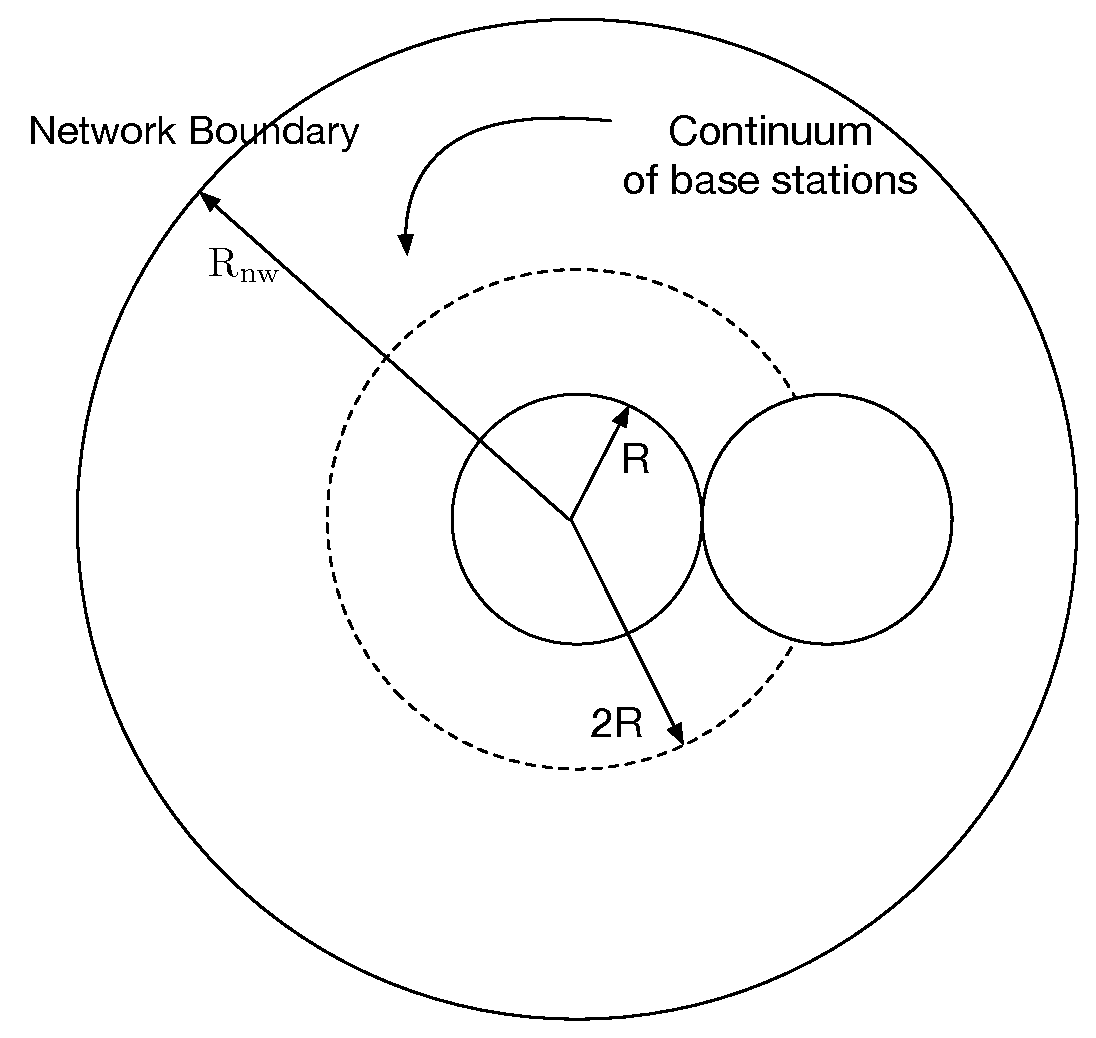
\includegraphics[width=0.7\linewidth, height=8cm]{Chapter6/Figures/fluid_model}
%	\caption{Fluid model illustration}
%	\label{fig:fluid_model}
%\end{figure}

\subsection{Lower bound of RNTI Consumption}
\label{sec:lower_bound_rnti}
Let $C_{\text{min}}$ be the low bound of RNTI required in the coverage zone of an eNB.

\subsubsection{Our proposal}
In a system with our proposed multiple period polling service, the utilization of RNTI is in a persistent manner. Hence, the number of occupied RNTI (i.e. PRD-RNTI) depends on the amount of device $N_d$ served by the eNB and polling period. 

Recall that eNB provides $M$ available polling periods. The polling period is denoted by $T_{n}$, where $T_n = 2^n \cdot W \cdot T_f$. The number of devices with the same polling period is denoted by $g_{n}$. For polling period $T_n$, there exist $2^n$ available polling windows. Thus with $g_n$ device, it needs at least $\frac{g_n}{2^n}$ RNTI to satisfy all devices. Similarly, it should provide at least $C_{min}$ RNTI satisfying the following formula:  
\begin{align}	
 C_{\text{min}} = \sum_{n=0}^{M} \frac{g_n}{2^n} \label{eq:lower-bound}
\end{align}

\subsubsection{Random access method}
Once that RNTI is allocated, it will be occupied within time duration $T_{\text{timer}}$, which is the expiration time of RRC inactivity timer. Let $C_{\text{RNTI}}$ be the total occupied RNTI number within $T_{\text{timer}}$.

\begin{lemma}
	Given that each MTC device reporting period is $T$ whose distribution can be of any type, the number of deployed devices in a cell is $N_d$, $C_{\text{RNTI}}$ follows distribution and its intensity can be approximated by 
	\begin{align}
		\lambda_{C_{\text{RNTI}}}  &= N_{d} T_{\text{timer}} \mathbb{E} \left[ \frac{1}{T} \right],
	\end{align}
\end{lemma}

\begin{proof}
	 The arguments of the statement that $C_{\text{RNTI}}$ approximately follows Poisson distribution are as follows:
	\begin{itemize}[leftmargin=*, noitemsep]
		\item Each MTC device independently chooses a random moment to transmit data. 
		\item The expectation of reporting period $T$ is much larger than duration of random access procedure, thus the probability that one device occupies one RNTI (i.e. transmits a packet) is small.
		\item A large number of MTC devices are deployed in each eNB coverage area.
	\end{itemize}
	Thus, the aggregated traffic of all the deployed MTC devices and the occupied RNTI number, follow Poisson distribution.
	
	Let $\lambda_{C_{\text{RNTI}}}$ be the intensity of $C_{\text{RNTI}}$. The void probability $\mathbf{P} \left\lbrace  C_{\text{RNTI}} = 0  \right\rbrace$ is thus equal to $\exp(-\lambda_{C_{\text{RNTI}}})$, which allows to estimate $\lambda_{C_{\text{RNTI}}}$. Recall that $N_{d}$ is the amount of M2M devices deployed in each cell. Hence, the locations of M2M devices form a Binomial Point Process (BPP). Given that $N_d$ is large enough, the locations of devices can be well approximated by a two-dimensional Poisson Point Process $\Phi_m$ with spatial intensity $\lambda_m = N_d / \pi R_{eq}^2$.

	Consider a given M2M device with label $i$. Its reporting period is $T_i$. The probability $p$ that one RNTI is occupied by this device is $T_{\text{timer}}/T_i$. The void probability is thus:
	\begin{align}
		\label{eq:void_proba_step_1}
		\mathbf{P} \left\lbrace  C_{\text{RNTI}} = 0 \right\rbrace  = \mathbb{E} \left[ \prod_{r_i \in \Phi_m}^{} 1 -  \frac{T_{\text{timer}}}{T_i} \right] ,
	\end{align}
	where $r_i$ refers to distance between the considered device and eNB located at the origin, $T_i$ is a random variable whose distribution is unknown. The subscript $i$ can be omitted for the sake of readability. According to Campbell theory, \eqref{eq:void_proba_step_1} can be further simplified: 
	\begin{align}
		\label{eq:rnti_nb_void_proba}
		\mathbf{P} \left\lbrace  C_{\text{RNTI}} = 0  \right\rbrace  &= \mathbb{E}_{\Phi_m} \left[ \prod_{r \in \Phi_m}^{} \mathbb{E}_{T} \left[ 1 - \frac{T_{\text{timer}}}{T} \right] \right] \nonumber\\
		&= \exp\left\lbrace -\mathbb{E}_{T} \left[ \int_{0}^{R_{eq}} \frac{T_{\text{timer}}}{T} 2\pi r \lambda_m dr  \right] \right\rbrace \nonumber\\
		&= \exp\left\lbrace -\lambda_m \pi R_{eq}^2  T_{\text{timer}} \mathbb{E}_{T} \left[ \frac{1}{T}  \right] \right\rbrace \nonumber \\
		&= \exp\left\lbrace -N_{d} T_{\text{timer}} \mathbb{E}_T \left[ \frac{1}{T} \right]\right\rbrace. 
	\end{align}
	
	From \eqref{eq:rnti_nb_void_proba}, we deduce that the average of $C_{\text{RNTI}}$, i.e., the intensity of corresponding Poisson distribution, is:
	\begin{align}
		\lambda_{C_{\text{RNTI}}} &= N_{d} T_{\text{timer}} \mathbb{E} \left[ \frac{1}{T} \right],
	\end{align}
\end{proof}

Recall that $C_{\text{RNTI}}$  follows poisson distribution, the minimum number of RNTI required $C_{\text{min}}$ should satisfy the probability where $C_{\text{RNTI}}$ is less than $C_{min}$ is greater than a predefined threshold, for example $0.99$. Thus, the low bound of required RNTI $C_{\text{min}}$ can be calculated as follows:
\begin{align}	
\label{eq:low-bound-rach}
C_{\text{min}} &= \min \left\lbrace \mathbf{P} \{ C_{RNTI} < C_{min} \} \geq \text{Threshold} \right\rbrace \nonumber \\
&= \min \left\lbrace X: \sum_{n=0}^{X} \frac{\lambda ^ n }{ n! } e^{-\lambda} \geq \text{Threshold} \right\rbrace 
\end{align}






%With OFDMA on the downlink or with SC-FDMA on the uplink, there is no (or limited if we consider inter-carrier interference) intra-cell interference. The single-carrier frequency-division multiple access method that is implemented in the uplink of LTE-Advanced introduces additional requirements to performs cheduling. That is, the PRBs that the SFDS algorithm allocates for a UE must be continuous in the frequency domain. Thus, it is reasonable to assume that channel suffers multiple path fading.
%
%
%Our model, called the fluid model in [12], the central cell is modeled by a disk of radius Rc and is surrounded by several rings of interfering cells at distances $2nR_c (n =1, 2, ...)$. The network size can be expressed as $R_{nw} =(2N_c+1)R_c$, where $N_c$ represents the number of rings.



\subsection{Resource Blocks Consumption}
%Compared with traditional random procedure requiring at least messages exchanged before data transmission, our proposed service allows device directly sending data packet thus reduce the Resource Block consumption. In random access procedure, RACH preamble in step 1 consists of $XX$ bytes. RAR in step 2 consists of a temporary C-RNTI which holds $4$ bytes.Contention resultion identity in step 3/4 is usually made from S-TMSI and has $6$ bytes. In total, 
%For a small payload less than $100$ bytes, 
%% http://blog.sina.com.cn/s/blog_927cff010101926v.html
%RA preamble generally requires $6$ Resource Blocks.
%% http://wireless.itri.org.tw/MPFiles/M2-1409-LTE_MAC_Intro_PartII.pdf
%Overhead in RAR is $4$ bytes.
%Resolution contention identity in L2/L3 messages is It $5$ octets.
%Contention solution echo $5$ octets.
% Please add the following required packages to your document preamble:
% \usepackage{booktabs}
RB consumption is analyzed for message transmission from step.3 to step 10 in Fig.~\ref{fig:lte-ra}. The cases of downlink and uplink transmission are separately considered within the approximated fluid model. Since M2M application is uplink-centric, the packet transmission in the uplink convey both collected data and signaling messages, while the transmission in the downlink only contains signaling.
It should be noted the just RRC layer signaling messages is consider. Signaling related to control information related to RB allocations are ignored.

Let $L$ be the message size (at MAC layer) to be transmitted. We assume that the considered message should be transmitted within unit Transmission Time Interval (TTI, $1$ ms in LTE). Let $N_{\text{RB}}(L)$ be the number of RB pairs required to satisfy this requirement. We evaluate the average number of RB pairs $\overline{N_{\text{RB}}}(L)$ with which a given device can transmit this message within unit TTI in a hexagonal cell.

Since $N_{\text{RB}}(L)$ depends the transport block size (TBS) that one pair of RB can support. TBS itself is determined by the modulation coding scheme (MCS) that the device chooses. We assume that the device always selects the MCS which carries the most bits. The MCS (indicated by TBS index) and TBS are given in Tab.~\ref{tab:tbs}. We assume that the TBS and the number of RB has linear relationship, thus we take the second column in Tab.~\ref{tab:tbs} to calculate the capacity per RB.

\begin{table}[]
	\centering
	\caption{Transport Block Size with respect to TBS index and Number of RBs. Source:~\cite[Tab.~7.1.7.2.1-1]{lte-eutra-physical-layer}.}
	\label{tab:tbs}
	\begin{tabular}{@{}c|cccccccccc@{}}
		\toprule
		\multirow{2}{*}{$I_{\text{TBS}}$} & \multicolumn{10}{c}{$N_{\text{RB}}$}                                                                        \\ \cmidrule(l){2-11} 
		& $1$      & $2$      & $3$      & $4$      & $5$      & $6$      & $7$      & $8$      & $9$      & $10$     \\ \midrule
		$0$                               & $16$     & $32$     & $56$     & $88$     & $120$    & $152$    & $176$    & $208$    & $224$    & $256$    \\
		$1$                               & $24$     & $56$     & $88$     & $144$    & $176$    & $208$    & $224$    & $256$    & $328$    & $344$    \\
		$2$                               & $32$     & $72$     & $144$    & $176$    & $208$    & $256$    & $296$    & $328$    & $376$    & $424$    \\
		$3$                               & $40$     & $104$    & $176$    & $208$    & $256$    & $328$    & $392$    & $440$    & $504$    & $568$    \\
		$4$                               & $56$     & $120$    & $208$    & $256$    & $328$    & $408$    & $488$    & $552$    & $632$    & $696$    \\
		$\cdots$                          & $\cdots$ & $\cdots$ & $\cdots$ & $\cdots$ & $\cdots$ & $\cdots$ & $\cdots$ & $\cdots$ & $\cdots$ & $\cdots$ \\
		$26$                              & $712$    & $1480$   & $2216$   & $2984$   & $3752$   & $4392$   & $5160$   & $5992$   & $6712$   & $7480$   \\ \bottomrule
	\end{tabular}
\end{table}

\subsubsection{Downlink Resource Block Consumption}
Given that one message should be transmitted within one TTI, the downlink data rate should be greater than a threshold and there exists a minimum SNR requirement so that a given MCS can be used. Recall that the channel gain only depends on the distance between receiver and transmitter $r$ (fading and shadowing are averaged out), SNR $\Theta$ is a function with respect to $r$. Thus, the problem comes down to how to calculate the SNR threshold for each MCS and find the function between $\Theta$ and $r$. 

We use one modified Shannon formula adjusted by simulation results proposed in~\cite{mogensen2007lte}. This formula is as follows:
\begin{align}
	\label{eq:debit_with_respect_sinr}
	S &= \beta B \eta  \log_2 \left( 1 + \frac{\Theta}{\Theta_{\text{ref}}} \right),
\end{align}
where $S$ (with unit of bits per second) is the date rate, $\beta$ adjusts for the system bandwidth (BW) efficiency of LTE , $\Theta_{\text{ref}}$ adjusts for the SNR implementation efficiency of LTE. Parameter $B$ refers to the RB bandwidth, $\Theta$ is the received SNR. The factor $\eta$ is a correction factor. By inversing \eqref{eq:debit_with_respect_sinr}, we obtain the SNR threshold with respect to the data rate as follows:
\begin{align}
	\label{eq:sinr_threshold}
	\Theta &= \Theta_{\text{ref}} \left(  2^{\frac{S}{\beta B \eta  }} - 1 \right).
\end{align}

In terms of SNR, due to scheduling algorithm and OFDMA multiplexing, the eNB during a given TTI only transmits to a certain device. Thus, there is no intra-cell interference. The interfering sources are other transmitting eNB. 
Actually, no closed form expression between SNR and distance is available in the case hexagonal cell. However, we can use one approximated expression with high accuracy in a fluid model. Proposed in ~\cite{kelif2010fluid}, SNR $\Theta$ can be expressed as follows:
\begin{align}
	\label{eq:snr_r_formula_in_fluid_model}
	\Theta &= \frac{\gamma-2}{2\pi \rho_{\text{eNB}} r^{\gamma}} (2R_c - r)^{\gamma - 2},
\end{align}
where $\rho_{\text{eNB}}$ is the eNB density in the fluid model, $R_c$ is the half intersite distance in the fluid model, $\gamma$ is the path-loss exponent.

To approximate the hexagonal network by a fluid model, according to~\cite{kelif2010fluid}, with substitution $\rho_{\text{eNB}} = 2/(3\sqrt{3} R_h^2)$, $R = \sqrt{3}R_h/2$ into \eqref{eq:snr_r_formula_in_fluid_model}, we have:  
\begin{align}
	\label{eq:sinr_with_repsect_distance}
	\Theta &= \frac{\sqrt{3} \left( \gamma - 2\right) }{4\pi} 
	\frac{(1 -\frac{r}{\sqrt{3} R_h})^{\gamma - 2}}{(\frac{r}{\sqrt{3}R_h})^{\gamma}}, \nonumber\\
	&= \frac{\sqrt{3} \left( \gamma - 2\right) }{4\pi} 
	\frac{(1 -\sqrt{  \frac {\sqrt{3}  }{  2\pi  }  }\frac{r}{R_{eq}})^{\gamma - 2}}{(\sqrt{  \frac {\sqrt{3}  }{  2\pi  }  }\frac{r}{R_{eq}})^{\gamma}}, 
\end{align}
From \eqref{eq:sinr_with_repsect_distance}, we deduce that $N_{\text{RB}}$ is a function of $L$ and $\frac{r}{R_{eq}}$, denoted as $N_{\text{RB}}(L, \nu)$.

Numerically inversing \eqref{eq:sinr_with_repsect_distance} with SNR threshold obtained via \eqref{eq:sinr_threshold}, we obtain the maximum distance to cell center that one device can be located if it need to satisfy the SNR threshold. Combing MCS and TBS mapping table, the coverage area of the central eNB can be divided into a series of $M$ rings in which the device can use the same amount of RBs. Hence, $N_{\text{RB}}(L, \nu)$ is a increasing step function with respect to relative location $\nu$ if $L$ is given.

Now we integrate $N_{\text{RB}}(L, r/R_h)$ on a disk cell with radius $R_{eq}$ equivalent to a hexagonal one to obtain the average number of RB pair consumption $\overline{N_{\text{RB}}}(L)$. The area of a cell is $1/\rho_{\text{eNB}} = \pi R_{eq}^2$ with $R_{eq} = R_c \sqrt{2\sqrt{3}/\pi} = R_h \sqrt{3\sqrt{3}/\left( 2\pi\right) } $. As the eNBs are uniformly distributed over the equivalent disk, the probability density (PDF) of $r$ is: $f_{r} (x) = 2x / R_{eq}^2, x \in \left[ 0, R_{eq}\right] $. Hence, $\overline{N_{\text{RB}}}(L)$ can be expressed as follow: 
\begin{align}
	\label{eq:avg_RB_nb_downlink}
	\overline{N_{\text{RB}}}(L)  &= \int_{0}^{R_{eq}} N_{\text{RB}}(L, \nu) \frac{2r}{R_{eq}^2}  dr \nonumber\\
	&=  \int_{0}^{R_{eq}} N_{\text{RB}}(L, \nu)  d (\frac{r}{R_{eq}})^2,
\end{align}

Recall that $N_{\text{RB}}(L,\nu)$ is a step function that can be written as $M$ linear combination of indicator functions of intervals. 
Let $N_{\text{RB}}(L, \nu, i)$ be the possible discrete values, $\nu_{\text{u,i}}$ and $\nu_{\text{l,i}}$ be the upper and low bound of interval with index $i, i =0, 1, ..., M-1 $. Thus, integral in \eqref{eq:avg_RB_nb_downlink} can be further written as follows:
\begin{align}
\label{eq:avg_RB_nb_downlink_final}
\overline{N_{\text{RB}}}(L) &= \sum_{i=0}^{M} N_{\text{RB}}(L, \nu, i) \left[ \nu_{\text{u,i}}^{2} - \nu_{\text{l,i}}^{2}\right],
\end{align}


\subsubsection{Uplink Resource Block Consumption}
Similar methodology presented in previous section can be applied to estimate the average number of RB pairs consumption for packet transmission in the uplink direction. The only difference relies in that function between SNR received at the eNB $\Theta_{\text{uplink}} $ and distance $r$ between device and eNB is different from \eqref{eq:sinr_with_repsect_distance}, since the fractional power control is taken into account in the uplink channel.

Due to the packet scheduling algorithms and SC-FDMA multiplexing, within a given TTI, only one device is transmitting to its attached eNB. The interfering sources are those transmitting devices in other cells and internal interference is null. Thus, the device intensity in the fluid model $\rho_{m} $ is identical to that of eNB. In reference~\cite{coupechoux2011set}, uplink interference analysis with fractional power control in LTE network is conducted within fluid model. The SNR expression for the uplink is as follows:
\begin{align}
\label{eq:sinr_with_repsect_distance_uplink}
\Theta_{\text{uplink}} = \frac{r^{-\gamma(1 - \alpha)}}{ 2 \pi \rho_{m} \sum_{n=1}^{\infty} (2nR)^{\alpha \gamma +2 - \gamma } I_{n}\left( \alpha, \gamma\right) },
\end{align}
where $\gamma$ is the path loss exponent, $\alpha$ is the power compensation factor that is adjusted between $\left[ 0, 1\right] $, $I_{n}\left( \alpha, \eta\right) = \int_{0}^{\frac{1}{2n}} x^{\alpha \gamma} \left[ (1-x)^{1-\gamma} +  (1 +x)^{1 - \gamma} \right] dx$. 

To approximate the hexagonal network by a fluid model, with substitution $\rho_{m} = 2/(3\sqrt{3} R_h^2)$, $R_c = \sqrt{3}R_h/2$ into \eqref{eq:sinr_with_repsect_distance_uplink}, we have:  
\begin{align}
	\label{eq:snr_distance_uplink}
	\Theta_{\text{uplink}} = \frac{\sqrt{3} (\frac{\nu}{\sqrt{3}})^{-\gamma(1 - \alpha)}}{ 4\pi \sum_{n=1}^{\infty} n^{\alpha \eta +2 - \eta} I_{n}\left( \alpha, \eta\right) },
\end{align}
where $\nu = r/ R_h$ is the relative location.

From \eqref{eq:sinr_threshold}, \eqref{eq:snr_distance_uplink} and TBS and MCS mapping table, we can get the step function $N_{\text{RB}}(L,\nu)$ for uplink data transmission, and use \eqref{eq:avg_RB_nb_downlink_final} to calculate average value. 


\subsection{Uplink Energy efficiency}
Energy efficiency is defined as the ratio between the data packet size and the consumed energy during a uplink reporting procedure. Note that the consumed energy is composed by two parts: consumption by uplink signaling message and data packet.
\begin{align}
	\overline{EE}_{\text{con}} &= L_0/\int_{0}^{R_{eq}} \sum_{j=0}^{M}\overline{N_{\text{RB}}}(L_j, r/R_{eq}) \frac{P_{\text{target}} (Kr^{\gamma})^{\alpha} L_j}{\beta B \eta  \log_2 \left( 1 + \frac{\Theta}{\Theta_{\text{ref}}} \right)} \frac{2r}{R_{eq}^2}dr \nonumber\\
	&= L_0/2 K^{\alpha} R_{eq}^{\alpha\gamma} P_{\text{target}} \sum_{j=0}^{M} \int_{0}^{R_{eq}} \overline{N_{\text{RB}}}(L_j, r/R_{eq}) \frac{ L_j x^{\gamma\alpha + 1} }{\beta B \eta  \log_2 \left( 1 + \frac{\Theta}{\Theta_{\text{ref}}} \right)} dx
\end{align}

\begin{align}
	\overline{EE}_{\text{polling}} &= L_0 / \int_{0}^{R_{eq}} \overline{N_{\text{RB}}}\left( L_0, r/R_{eq}\right) \frac{ P_{\text{target}} L_0}{\beta B \eta  \log_2 \left( 1 + \frac{\Theta}{\Theta_{\text{ref}}} \right)} \frac{2r}{R_{eq}^2}dr \nonumber\\
	&= 1 / 2 K^{\alpha} P_{\text{target}} \int_{0}^{1} \overline{N_{\text{RB}}}\left( L_0, x \right) \frac{ R_{eq}^{\alpha \gamma} x^{\alpha \gamma} }{\beta B \eta  \log_2 \left( 1 + \frac{\Theta}{\Theta_{\text{ref}}} \right)} x d x \nonumber \\
	&= 1/ 2 K^{\alpha} R_{eq}^{\alpha \gamma} P_{\text{target}} \int_{0}^{1} \overline{N_{\text{RB}}}\left( L_0, x \right) \frac{  x^{\alpha \gamma + 1} }{\beta B \eta  \log_2 \left( 1 + \frac{\Theta(x)}{\Theta_{\text{ref}}} \right)} d x
\end{align}
where $P_t$ is the transmitted power on one RB, $\Theta(x)$ is given by ~\eqref{eq:snr_distance_uplink} for uplink.
